\section{App management}
\label{sec:app_management}

\subsection{Requirements}
\label{sec:appman_requirements}

As shown in \autoref{fig:state_diagram} in \autoref{sec:design_overview}, the ``no app selected''-state and the ``no child selected''-state are the states which the launcher is in when the user is about to launch a \giraf[] app. \\

\noindent Three pieces of information are needed in order to launch an app:

\begin{enumerate}
	\item the current authenticated guardian
	\item the app to launch
	\item the selected child to launch the app with
\end{enumerate}

The first requirement is already given, since the launcher cannot be in any of the two states without the user already being authenticated.
The second requirement is straightforward, as it is not possible to launch an app without knowing which app to launch.
The first and third requirements are needed in order to fulfill the services which the launcher needs to have in order to be a functional part of the \giraf[] platform, as shown in \autoref{fig:external_architecture}.

\todo{tilfoej krav om hvorfor vi skal vise ugenr/date, og network connectivity}

\subsection{Solution}
\label{sec:appman_solution}



\autoref{fig:appmanagement_design} shows the flowchart over the interactions the user can perform, and the actions the launcher takes upon the interactions, in order to fullfill the requirements listed in \autoref{sec:appman_requirements}.


\begin{figure}[h]
	\centering
	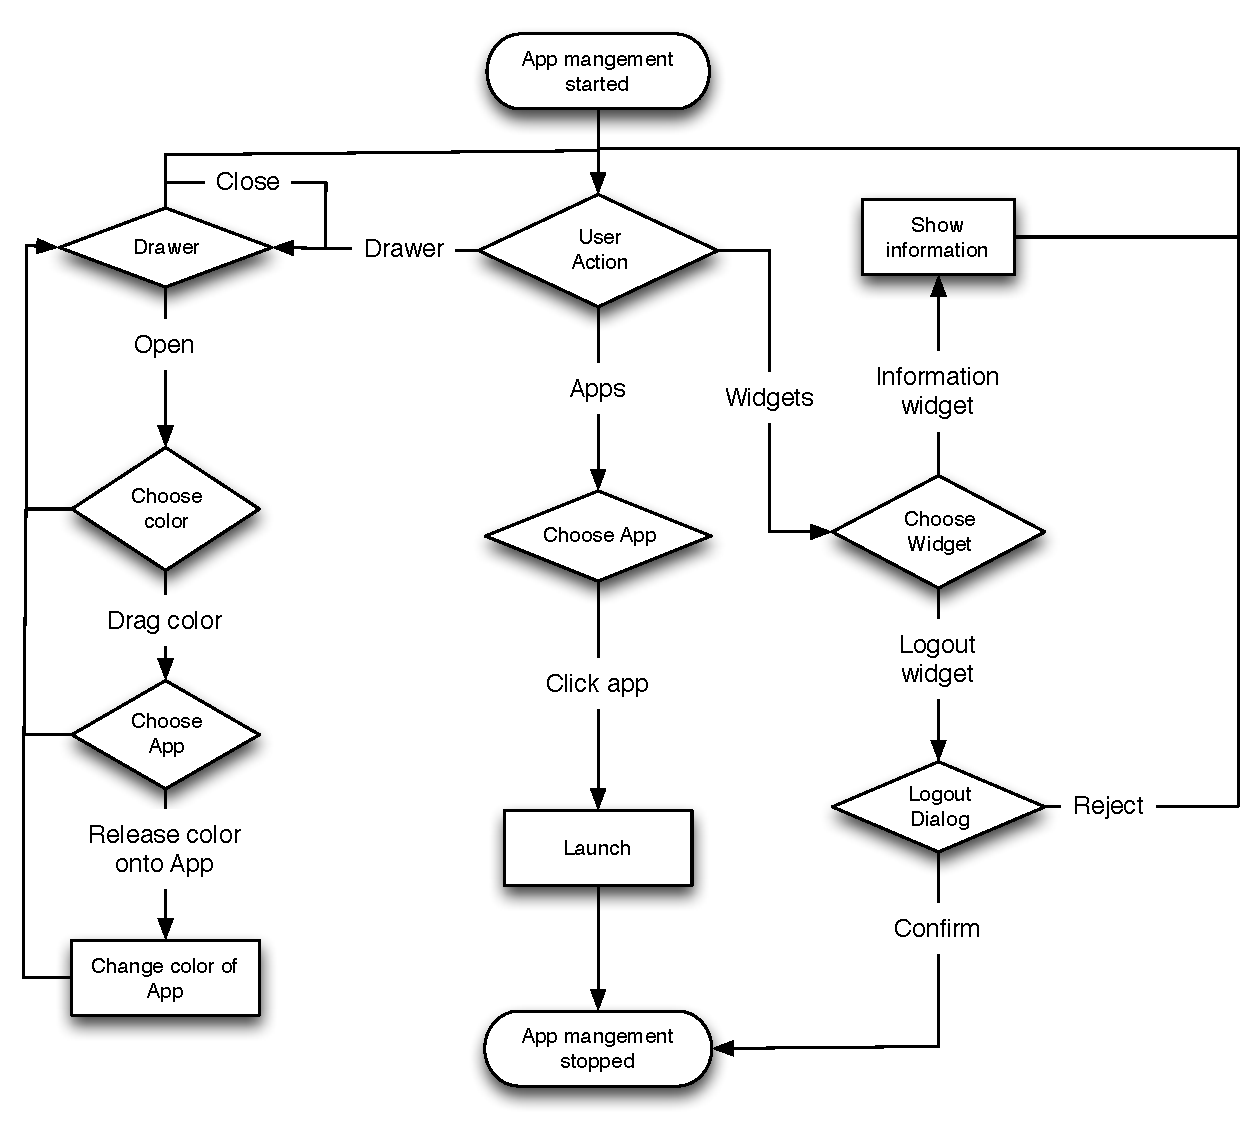
\includegraphics[width=1\textwidth]{gfx/appmanagement.pdf}
	\caption{Flowchart over the app management functionality}
	\label{fig:appmanagement_design}
\end{figure}








\subsubsection{The drawer}
\label{sec:drawer}
\paragraph{Widgets}
\label{par:widgets}
\paragraph{Color picker}
\label{par:colorpicker}